\documentclass[11pt]{article}

% "preprint" prints the author and page numbers. "final" drops the page numbers.
\usepackage[preprint]{acl}

\usepackage{times}
\usepackage{latexsym}
\usepackage[T1]{fontenc}
\usepackage[utf8]{inputenc}
\usepackage{microtype}
\usepackage{inconsolata}
\usepackage{graphicx}
\usepackage{makecell}

\graphicspath{{figures/}}

\title{Detecting LLM-Written Code on AIGCodeSet: Tuned Code Encoders versus N-gram Baselines}

\author{Andreas Bartsiokas \\
  LT2326 Machine Learning \\
  October 2026}

\begin{document}
\maketitle

\begin{abstract}
In this project I look at whether code written by an LLM can be told apart from human-written code, and which LLM wrote it, using the AIGCodeSet dataset. I compare word and character n-gram logistic regression with fine-tuned code encoders (CodeBERT, GraphCodeBERT, UniXcoder) on four task variants, with splits grouped by problem and a test set that was used only once. On dev, a tuned character n-gram baseline does better than CodeBERT and GraphCodeBERT. A tuned UniXcoder beats the baseline on all four variants, but the difference is statistically clear only for binary detection. Averaging six seeds and mixing the result with the baseline improves the scores a bit more. Most errors come from two places: code that an LLM \emph{edited} from a human submission (detected only 27--54\% of the time, against 94--98\% for code written from scratch), and Gemini, whose from-scratch code is often classified as human. In an ablation of the character baseline, identifier names turn out to be the strongest cue.
\end{abstract}

% ---------------------------------------------------------------------------
\section{Introduction}
\label{sec:intro}

Telling LLM-generated code apart from code written by students or competitive programmers is hard to do just by looking at it. This has been in the spotlight for the last couple of years: professors worry about students handing in AI-written work, and in industry many companies adopt AI tools while others enforce strict no-AI policies. I approach the problem empirically, with three questions: (i) How well do cheap lexical baselines and fine-tuned code encoders do when the split never shares a programming problem between train and test? (ii) Which hyperparameters and cues actually matter? (iii) Where do the models fail? This is my own evaluation and not a replication. The dataset paper \citep{demirok-kutlu-2025-aigcodeset} reports binary detection with classical classifiers on a random split, so my numbers cannot be compared with theirs directly. Recent work also shows that detection results depend a lot on the evaluation setting, and that they get worse under more realistic conditions, such as unseen generators, code written partly by humans and partly by AI, edited code, and distribution shift \citep{orel-etal-2026-aicd,demirok-etal-2026-multiaigcd}.

% ---------------------------------------------------------------------------
\section{Data}
\label{sec:data}

AIGCodeSet \citep{demirok-kutlu-2025-aigcodeset} pairs human solutions from CodeNet \citep{puri-etal-2021-codenet} with code from three LLMs (CodeLlama 34B, Codestral 22B and Gemini 1.5 Flash). The LLM code comes in two kinds: either the LLM writes a solution from scratch (\emph{generate}), or it \emph{edits} a human submission to fix a runtime error or a wrong output. This difference matters, because both AIGCodeSet and MultiAIGCD find that AI-edited code is much harder to detect than code generated from scratch \citep{demirok-kutlu-2025-aigcodeset,demirok-etal-2026-multiaigcd}. After deduplication I keep 7,531 samples and split them by problem into train (5,267), dev (739) and test (1,525), so no problem appears in more than one split. Some files have identical code under both labels (478 of them), and I remove those from every split, which leaves 4,953 train, 681 dev and 1,419 test files. Removing them makes the splits slightly easier than the raw data.

From this I build four task variants: \texttt{binary} (human vs AI) and \texttt{multiclass} (human, GEMINI, LLAMA, CODESTRAL) use all the data, while \texttt{binary\_generate} and \texttt{multiclass\_generate} drop the edited code. Table~\ref{tab:sizes} shows the test set sizes. The models only ever see a normalized copy of the code, with line endings unified, tabs expanded to spaces, and trailing spaces, leading blank space and final-newline differences removed. I did this because an audit of the raw files had found formatting quirks that give the source away (for example, 21\% of LLAMA files start with whitespace). No metadata column is given to the models.

\begin{table*}[t]
  \centering
  \small
  \begin{tabular}{lrl}
    \hline
    \textbf{Variant} & \textbf{Human} & \textbf{AI (per class)} \\
    \hline
    binary / multiclass                   & 905 & 514 (GEMINI 179, LLAMA 146, CODESTRAL 189) \\
    binary\_generate / multiclass\_generate & 905 & 186 (GEMINI 62, LLAMA 61, CODESTRAL 63) \\
    \hline
  \end{tabular}
  \caption{Test set sizes.}
  \label{tab:sizes}
\end{table*}

% ---------------------------------------------------------------------------
\section{Methods}
\label{sec:methods}

\paragraph{Baselines.}
My baselines are TF-IDF features with logistic regression, on either word or character n-grams, with balanced class weights. For the character model I picked n-grams (1,6) and C=10 with 7-fold cross-validation on the training folds only, capping the features at 300k. The word model just reuses C=10.

\paragraph{Encoders.}
I fully fine-tune three pretrained code encoders: CodeBERT \citep{feng-etal-2020-codebert}, GraphCodeBERT \citep{guo-etal-2021-graphcodebert} and UniXcoder \citep{guo-etal-2022-unixcoder}. All of them use AdamW with a linear schedule and 10\% warmup, weight decay 0.01, batch size 16 and learning rate 2e-5, and train for 4 epochs without class weights. CodeBERT and GraphCodeBERT run at 128 tokens with the default dropout of 0.1, and I did not tune them further. Since half of the files are longer than 128 tokens, the final UniXcoder reads the first 256 tokens instead (in a two-seed test this gave about +.01, short of the tuning rule below), and it uses dropout 0.0 (\S\ref{sec:training}). I keep the checkpoint with the best dev macro-F1 at the end of an epoch. All models are trained on the train split only.

\paragraph{Tuning protocol.}
I tuned on the two generate variants with seeds 0--2. A change was kept only if it raised the mean dev score by at least .01 on both variants, and at most one of the six paired seed comparisons went the other way. The dev set is small (only 93 AI files in \texttt{binary\_generate} and 31 per class in \texttt{multiclass\_generate}), so I treat differences below about .03 between single runs as ties. The final models use fresh seeds 3--8, and each run is evaluated on test only once.

\paragraph{Ensembles and statistics.}
The \emph{seed ensemble} averages the class probabilities of the six UniXcoder runs. The \emph{mix} then averages the ensemble with the character baseline at a weight of 0.5. I did not choose this weight on dev (I only looked at 0.3 and 0.7 in some exploratory runs). To test the gap to the baseline I use a paired bootstrap over problems (1,000 resamples), so that files from the same problem stay together. The seeds are held fixed, so the intervals do not include variation between seeds. All scores are macro-F1.

% ---------------------------------------------------------------------------
\section{Results}
\label{sec:results}

\subsection{Final test results}
\label{sec:final-test}

UniXcoder beats the character baseline on all four variants (Table~\ref{tab:test}). However, a single model is significantly better only on \texttt{binary}. The seed ensemble is significantly better on three of the four, although only barely on \texttt{multiclass} and \texttt{binary\_generate}. The mix scores highest everywhere, but I only added it after seeing the dev results (where it was tied with the ensemble), so I report it as an extra column without an interval. On dev, the fresh seeds score close to the tuning seeds (.923 and .818 against .926 and .829 on the generate variants), so the tuning result is not just down to lucky seeds.

\begin{table*}[t]
  \centering
  \small
  \setlength{\tabcolsep}{4pt}
  \begin{tabular}{lccccccc}
    \hline
    \textbf{Variant} & \makecell{\textbf{char}\\\textbf{LogReg}} & \makecell{\textbf{word}\\\textbf{LogReg}} & \makecell{\textbf{UniXcoder,}\\\textbf{1 seed}} & \makecell{\textbf{Seed}\\\textbf{ensemble}} & \makecell{\textbf{Mix}\\\textbf{0.5}} & \makecell{\textbf{1 seed}\\\textbf{$-$ char}} & \makecell{\textbf{Ensemble}\\\textbf{$-$ char}} \\
    \hline
    binary              & .743 & .658 & .772 $\pm$ .002 & .778 & .783 & +.029 [+.011, +.048]   & +.034 [+.015, +.054] \\
    multiclass          & .554 & .477 & .571 $\pm$ .026 & .595 & .614 & +.017 [$-$.016, +.052] & +.041 [+.003, +.077] \\
    binary\_generate     & .923 & .885 & .939 $\pm$ .008 & .943 & .948 & +.016 [$-$.003, +.035] & +.020 [+.001, +.041] \\
    multiclass\_generate & .808 & .772 & .837 $\pm$ .016 & .839 & .867 & +.029 [$-$.006, +.066] & +.031 [$-$.008, +.070] \\
    \hline
  \end{tabular}
  \caption{Test macro-F1. UniXcoder single seed is mean $\pm$ std over 6 seeds. The intervals are 95\% bootstrap intervals for the difference from the character baseline.}
  \label{tab:test}
\end{table*}

\subsection{What mattered in training}
\label{sec:training}

At 128 tokens on dev, the choice of pretrained checkpoint made the biggest difference: UniXcoder scored .896 / .778, GraphCodeBERT .869 / .739 and CodeBERT .834 / .712 (\texttt{binary\_generate} / \texttt{multiclass\_generate}), and UniXcoder beat GraphCodeBERT in all six paired seed comparisons. This fits with recent benchmarks, which also find large differences between code encoders and newer transformer models on AI-code detection \citep{orel-etal-2026-aicd}. CodeBERT and GraphCodeBERT were never evaluated on test. Inverse-frequency class weights hurt the multiclass task (CodeBERT on \texttt{multiclass}: .404 with weights against .515 without), because they flooded the human-heavy dev set with false AI predictions.

\begin{table*}[t]
  \centering
  \small
  \begin{tabular}{lcc}
    \hline
    \textbf{Setting} & \textbf{binary\_generate} & \textbf{multiclass\_generate} \\
    \hline
    dropout 0.1 (starting point)                            & .906                  & .798 \\
    \textbf{dropout 0.0}                                    & \textbf{.926}         & \textbf{.829} \\
    dropout 0.2                                             & .862                  & .751 \\
    dropout 0.0, 6 epochs                                   & .930                  & .815 \\
    dropout 0.0, batch 8 / 32                               & .924 / .921           & .819 / .803 \\
    dropout 0.0, weight decay 0.1                           & .921                  & .821 \\
    dropout 0.1: 384 tokens / lr 3e-5 / lr 1e-5 (6 epochs)  & .911 / .904 / .901    & .774 / .793 / .780 \\
    \hline
  \end{tabular}
  \caption{UniXcoder, 256 tokens, dev macro-F1, seeds 0--2.}
  \label{tab:tuning}
\end{table*}

Out of all the changes in Table~\ref{tab:tuning}, only removing dropout gave a consistent gain across all six paired seeds. On \texttt{binary\_generate}, the training loss drops close to zero while dev F1 barely moves after the second epoch (Figure~\ref{fig:curves}). On the small multiclass dev set, dev F1 still moves by .02--.04 between neighbouring epochs.

\begin{figure}[t]
  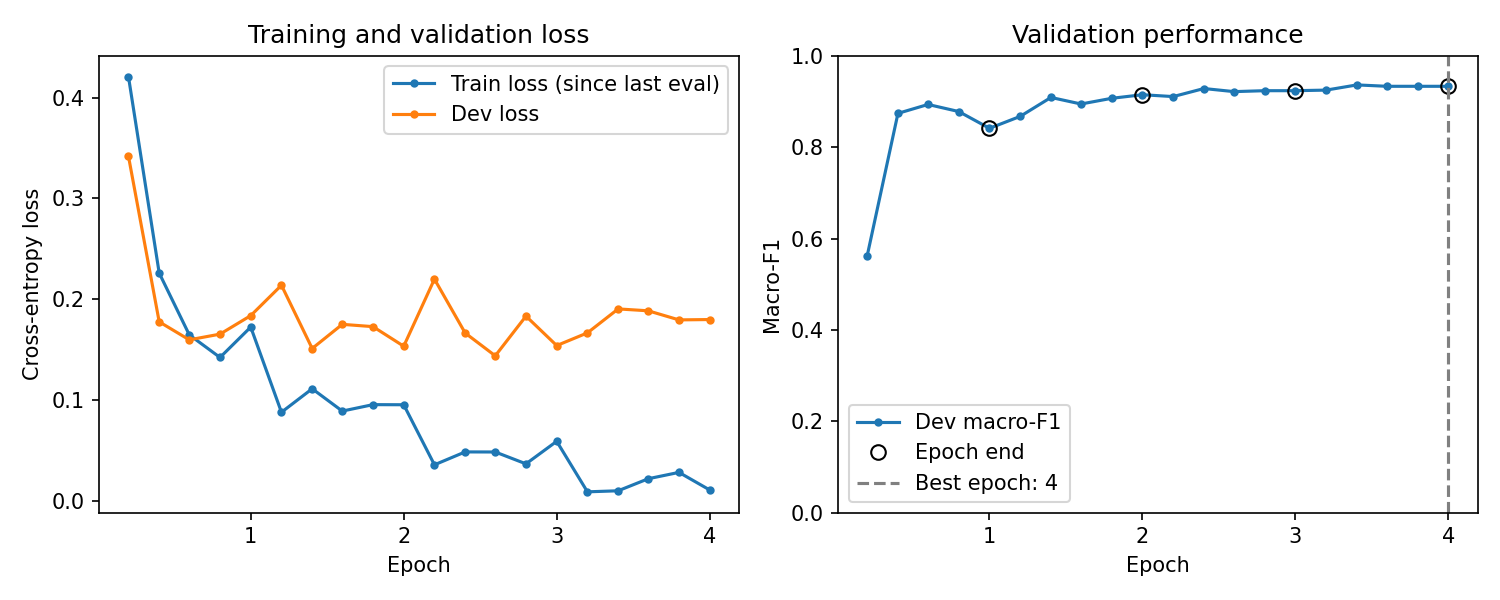
\includegraphics[width=\columnwidth]{training_curves_seed5_binary_generate.png}
  \caption{Training curves of UniXcoder, seed 5, \texttt{binary\_generate}, dev macro-F1 and loss, 5 evaluations per epoch.}
  \label{fig:curves}
\end{figure}

\subsection{Which cues carry the signal}
\label{sec:cues}

To see which cues the character baseline relies on, I ran an ablation on its input, removing the layout or the comments, or masking the identifier names (7-fold CV on the training folds, generate variants only).

\begin{table}[t]
  \centering
  \small
  \begin{tabular}{lcc}
    \hline
    \textbf{Input} & \makecell{\textbf{binary\_}\\\textbf{generate}} & \makecell{\textbf{multiclass\_}\\\textbf{generate}} \\
    \hline
    full code               & .909 & .791 \\
    layout removed          & .907 & .778 \\
    comments removed        & .902 & .787 \\
    identifier names masked & .882 & .765 \\
    \hline
  \end{tabular}
  \caption{Macro-F1 mean over folds.}
  \label{tab:ablation}
\end{table}

Masking identifiers costs the most (about .026, Table~\ref{tab:ablation}), but that is only about one standard deviation across folds, so the ablations rank the cues rather than show significant effects. Many of the top n-grams of the full model are pieces of names, like \texttt{\_}, \texttt{get\_} and \texttt{min\_} (Figure~\ref{fig:ngrams}). Still, most of the signal survives name masking, which suggests that no single cue explains detection on its own. The ablations are also not additive, and they only show how much a cue contributes, not which class it points towards. My experiments cannot tell whether the encoders use the same cues.

\begin{figure}[t]
  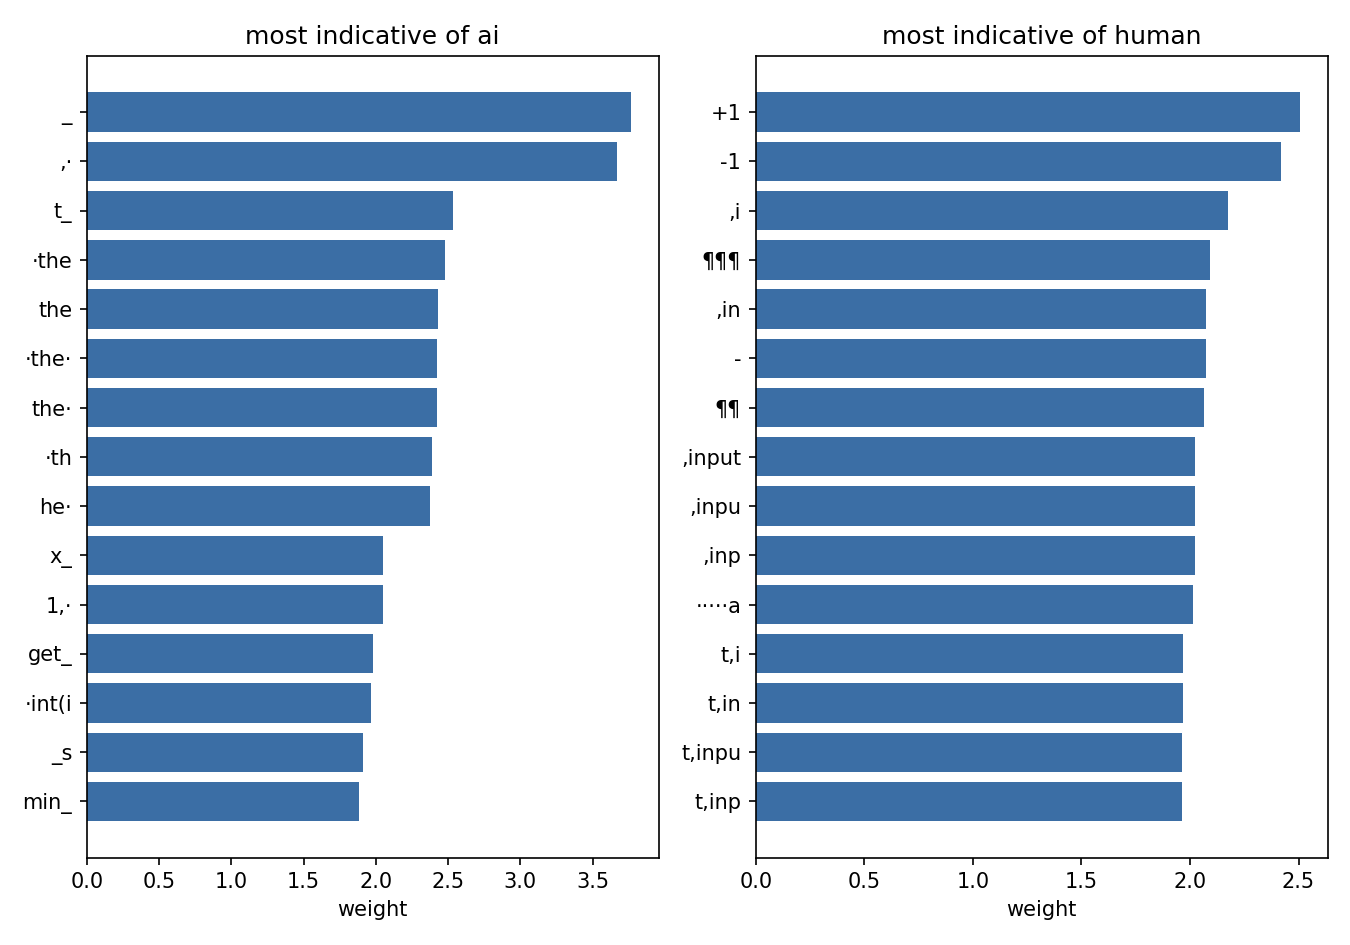
\includegraphics[width=\columnwidth]{top_features_char_binary_generate.png}
  \caption{Top character n-grams of the char LogReg, \texttt{binary\_generate}. \textperiodcentered{} is a space, \P{} a newline.}
  \label{fig:ngrams}
\end{figure}

\subsection{Where the models fail}
\label{sec:errors}

\begin{table}[t]
  \centering
  \small
  \setlength{\tabcolsep}{5pt}
  \begin{tabular}{lrrr}
    \hline
    \textbf{True source} & \textbf{n} & \makecell{\textbf{UniXcoder}\\\textbf{ensemble}} & \makecell{\textbf{char}\\\textbf{LogReg}} \\
    \hline
    Human (false positives) & 905 & 9.9\%  & 8.7\% \\
    LLAMA, generate         & 61  & 98.4\% & 98.4\% \\
    CODESTRAL, generate     & 63  & 98.4\% & 92.1\% \\
    GEMINI, generate        & 62  & 93.5\% & 90.3\% \\
    LLAMA, edit             & 85  & 54.1\% & 43.5\% \\
    CODESTRAL, edit         & 126 & 54.0\% & 35.7\% \\
    GEMINI, edit            & 117 & 27.4\% & 22.2\% \\
    \hline
  \end{tabular}
  \caption{Share of files detected as AI, by true source, \texttt{binary}, test.}
  \label{tab:breakdown}
\end{table}

Edited code is the main source of error (Table~\ref{tab:breakdown}). It makes up 328 of the 514 AI files in \texttt{binary}, and it is detected far less often than code written from scratch, which explains most of the gap between \texttt{binary} (.78) and \texttt{binary\_generate} (.94). This is in line with both AIGCodeSet and MultiAIGCD, where AI-edited code is also harder to detect than code generated from scratch \citep{demirok-kutlu-2025-aigcodeset,demirok-etal-2026-multiaigcd}. In \texttt{multiclass\_generate}, the ensemble predicts Human for 37\% of the GEMINI files, but another LLM for only 8\% (LLAMA 2\%, CODESTRAL 6\%). Figure~\ref{fig:confusion} shows a single seed rather than the ensemble. So Gemini is hard because its code looks human to the models, not because it looks like the other two LLMs. When the code is written from scratch, telling the LLMs apart mostly works: F1 is .91 (LLAMA), .82 (CODESTRAL) and .64 (GEMINI) for the ensemble, and .96, .86 and .67 for the mix. The original AIGCodeSet paper \citep{demirok-kutlu-2025-aigcodeset} also reports lower recall for code generated by Gemini than by CodeLlama or Codestral. Finally, on the full data about 1 in 10 human files gets flagged as AI.

\begin{figure}[t]
  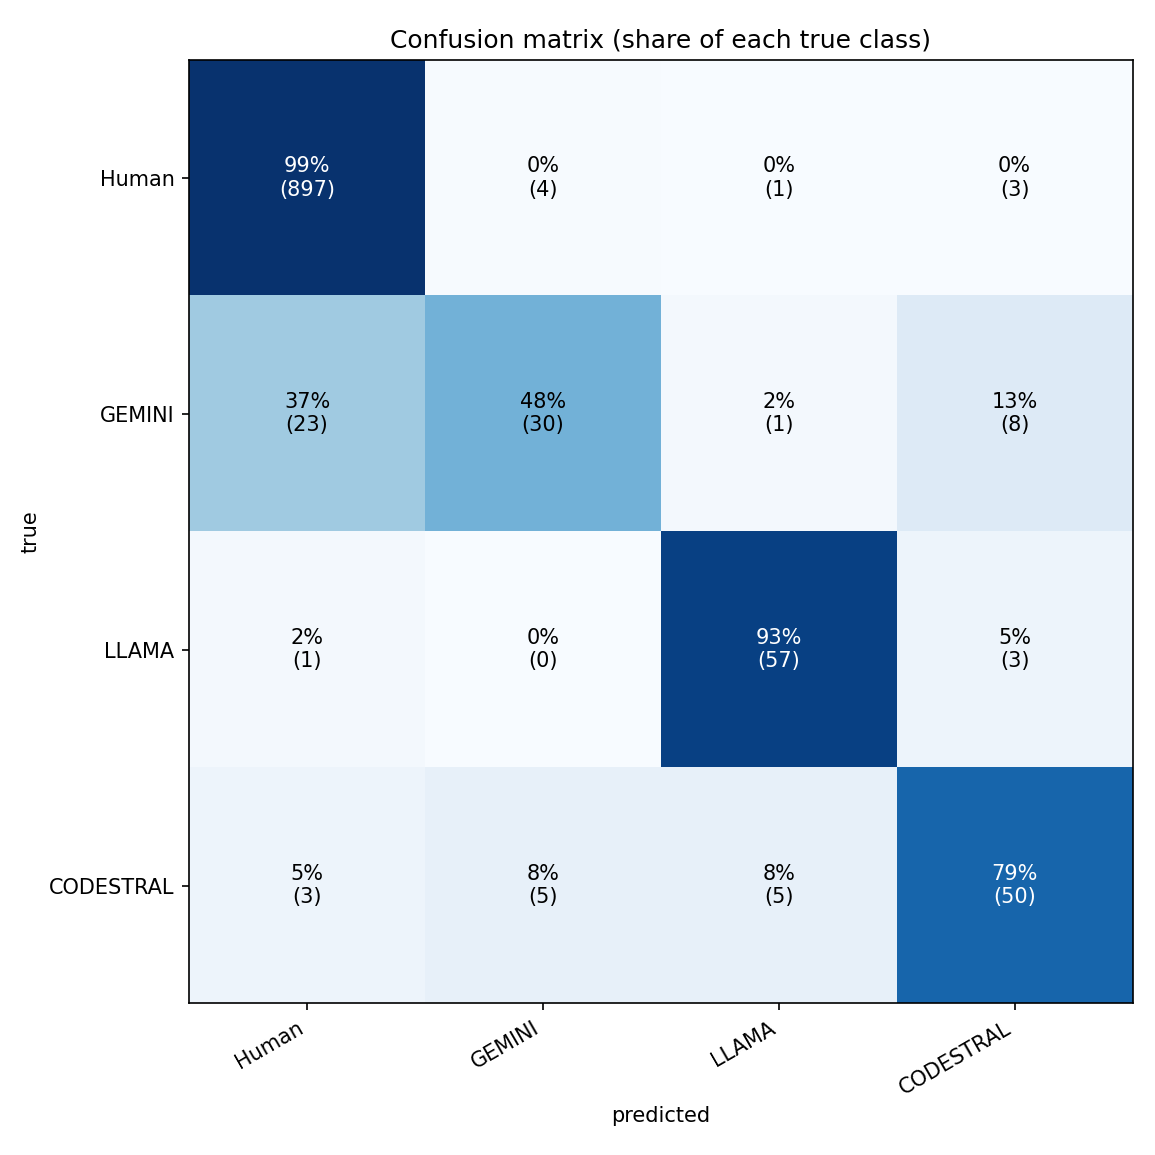
\includegraphics[width=\columnwidth]{confusion_matrix_seed3_multiclass_generate.png}
  \caption{Confusion matrix, UniXcoder seed 3, \texttt{multiclass\_generate}, test.}
  \label{fig:confusion}
\end{figure}

% ---------------------------------------------------------------------------
\section{Discussion}
\label{sec:discussion}

\paragraph{Supported by my results.}
(1) A tuned character n-gram model is a strong baseline, and CodeBERT and GraphCodeBERT do not reach it on dev under a problem-grouped split. (2) UniXcoder without dropout is at least as good on every variant, and clearly better on \texttt{binary}. (3) Averaging seeds gives a small but reliable gain, and combining the encoder with the n-gram model gave the best test scores. (4) Edited code and Gemini are the hardest cases. Point (4) closely matches AIGCodeSet: there too, performance varies a lot between generation scenarios, and Gemini's code is generally harder to spot than CodeLlama's or Codestral's \citep{demirok-kutlu-2025-aigcodeset}. It also agrees with MultiAIGCD, which finds much lower performance on AI-edited code than on code generated from scratch, across several languages and detector architectures \citep{demirok-etal-2026-multiaigcd}.

\paragraph{Speculation, not tested.}
UniXcoder might do better than CodeBERT because of its pretraining objectives, but I did not run a pretraining ablation to check this. Dropout may hurt because the training set is small, although I only observed the effect and did not test why. The mix may help because the two models make different mistakes, which I did not measure directly. Finally, Gemini may simply write code that is closer to human style, but I did not analyse its style.

% ---------------------------------------------------------------------------
\section{Conclusion}
\label{sec:conclusion}

On AIGCodeSet, a tuned UniXcoder (dropout 0.0, 256 tokens) is ahead of the best n-gram baseline on every variant, with a clear margin on binary detection and smaller, mostly non-significant margins on the rest. Seed averaging and mixing with the baseline add a little on top. The hard cases are still edited code and Gemini. The most useful next steps would be an external human-only test set, to check false positives, and a split that holds out one LLM, to test how well the models generalize. This matches recent benchmark results: obviously AI-written code is no longer the main problem, but edited or hybrid code is, and so is keeping performance up under more realistic evaluation conditions \citep{orel-etal-2026-aicd,demirok-etal-2026-multiaigcd}.

% ---------------------------------------------------------------------------
\section*{Limitations}

\begin{itemize}
  \item The dev set is small, so tuning decisions on the multiclass variants are noisy. I compared about 20 configurations on dev. The fresh seeds score only .003--.011 lower there, which rules out lucky seeds, but not overfitting to dev.
  \item \texttt{binary} and \texttt{multiclass} reuse a configuration that was tuned on the generate variants only.
  \item The test sets are small for the LLM classes (61--63 files each in the generate variants), so several intervals include zero.
  \item I did not keep the cross-validation and ablation code, so Table~\ref{tab:ablation} cannot be re-run.
  \item I added the mix after seeing dev, and I did not tune its weight.
  \item Everything comes from a single data source: there is no out-of-distribution evaluation and no external human-only test set (such as MBPP).
  \item I did not run ModernBERT (the installed library was too old for it) or a larger code LLM with LoRA.
  \item I only use one dataset and one programming language, and recent benchmarks show that detector performance can vary a lot across languages, generators and evaluation scenarios \citep{orel-etal-2026-aicd,demirok-etal-2026-multiaigcd}.
\end{itemize}

\bibliography{coder_paper}

\end{document}
